\begin{center}
    \textbf{--------- Lezione 11 - 19 aprile 2021 ---------}
\end{center}

\section{Use Case: SmartWheels}
Quello che si vuole creare è un sistema per facilitare la navigazione outdoor per persone con disabilità motorie. 
Una persona a sedie a rotelle non può sapere in anticipo gli ostacoli che troverà durante il percorso.

Le app per navigazione outdoor (come Maps o Waze) dovrebbero personalizzare il percorso per queste persone in base alle barriere architettoniche che può trovare.
Attraverso queste app l'utente può settare ciò che preferisce evitare durante il percorso, tipo: 
\begin{itemize}
    \item small-step-up
    \item small-step-down
    \item medium-step-up
    \item medium-step-down
\end{itemize}
Il sistema calcola il percorso secondo le preferenze scelte.
Ci sono sistemi simili, ma la raccolta di dati annotati (urban features UF come barriere architettoniche, rampe, ecc.) è molto complicata. 
Le informazioni vengono raccolte tramite: 
\begin{itemize}
    \item crowdsourcing: è difficile che gli utenti in sedia a rotelle vogliano fornire dati mentre circolano. Viene collezionata solo una frazione di dati utili al sistema
    \item computer vision: efficiente per UF come strisce pedonali, ma non sempre efficienti per altre UF
\end{itemize}

Un metodo complementare è SmartWheels, un sistema in grado di rilevare, in modo automatico, gli ostacoli (come le barriere architettoniche) utilizzando sensori inerziali installati sulla sedie a rotelle e sfruttando metodi supervisionati di activity recognition. 

\subsection{Riconoscere attività vs UF}
L'idea è riconoscere le attività che rivelano la presenza di barriere architettoniche. Serve anche sapere dove si trova l'utente per sapere la posizione della barriera architettonica. 

Ci sono diversi tipi di sedie a rotelle che possono essere spinte dagli utenti stessi, da un'altra persona o da propulsione elettrica, ma SmartWheel è focalizzato su utenti in grado di spingere autonomamente la propria sedia a rotelle. 

In una fase iniziale si è definito il target di attività, quello che poi il classificatore dovrà riconoscere. Si è definita una gerarchia di UF dopo aver effettuato delle interviste.
\begin{center}
    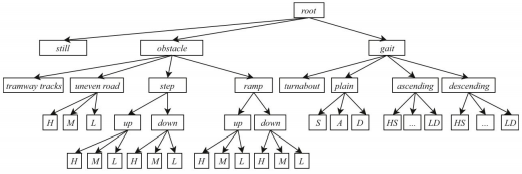
\includegraphics[width=\textwidth]{images/MobiDEV/6. activity recognition/smart wheel.PNG}
\end{center}
La radice indica qualsiasi UF, da cui vengono identificati gli altri sotto UF.


\subsection{Architettura del sistema}
\begin{center}
    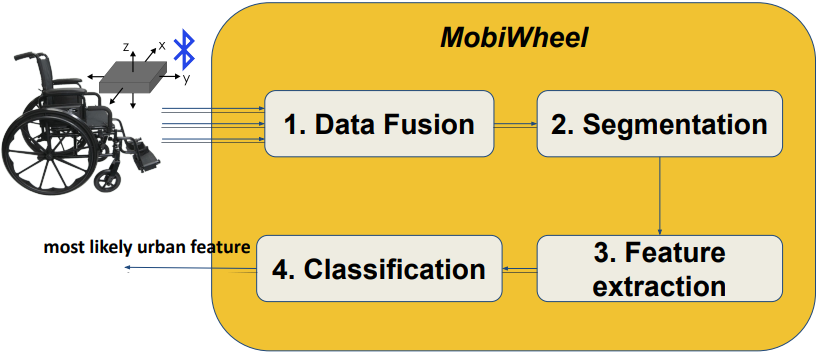
\includegraphics[width=.9\textwidth]{images/MobiDEV/6. activity recognition/smart wheel - architettura.PNG}
\end{center}
I sensori inerziali tramite bluetooth comunicano al sistema di riconoscimento.
Nel data fusion vengono allineati i dati che arrivano dai diversi dispositivi in modo tale da effettuare la segmentazione (fatta tramite la tecnica di sliding window).
Con le finestre temporali, estraiamo le features ovvero la rappresentazione numeri dei segmenti temporali. Forniamo al classificatore il vettore in modo tale che ci dia la UF più probabile.

\subsubsection{Acquisizione del dataset}
I dati sono stati acquisiti in un'organizzazione no-profit che ha messo a disposizione la sua area di allenamento con ostacoli urbani, come i gradini. 
17 utenti in sedia a rotelle hanno seguito un percorso predefinito mentre venivano registrati, alcuni in ambiente controllato (una specie di palestra), altri in strada. 

Sono stati usati 3 piccole board che comunicano ad uno smartphone tramite BLE (bluetooth low energy). 
Gli utenti dispongono di uno smartwatch sul polso e uno smartphone, in una fascia da braccio, sulla gamba. 
Poi un'app mobile colleziona e salva internamente questi dati.

La prima fase è allineare i dati, presi da ciascun dispositivo sui tre assi, temporalmente. 
Successivamente viene effettuata la segmentazione a sliding window ad un certo overlap. 

Un problema è che alcune attività richiedono poco tempo (come scendere uno scalino), altre invece sono più lunghe (come un'andatura su piano).
C'è il problema che nel segmento viene riconosciuta l'attività prevalente, in questo caso non viene riconosciuta l'attività del gradino. 
Una soluzione è dare priorità ad UF attraversabili in breve tempo, oppure ridurre la sliding window, ma questo avrebbe aumentato la complessità computazionale. 

I classificatori principalmente investigati sono:
\begin{itemize}
    \item Random Forest
    \item Hierarchical Random Forest: una versione gerarchica del Random Forest
\end{itemize}

Tramite la leave-one-subject-out cross validation sono stati determinati i migliori parametri.
